\documentclass[12pt]{article}
\usepackage{amsmath, amssymb, geometry, tikz, graphicx}
\geometry{a4paper, margin=1in}
\usepackage{hyperref}

\title{Polynomial Functions}
\author{}
\date{}

\begin{document}

\maketitle

\section*{Learning Objectives}
\begin{itemize}
  \item Understand the definition and structure of polynomial functions.
  \item Determine whether a given function is a polynomial.
  \item Analyze end behavior based on degree and leading coefficient.
  \item Identify domain, range, and symmetry of polynomials.
  \item Locate zeros and determine positive/negative intervals.
\end{itemize}

\section{Definition and Structure}
A \textbf{polynomial function} is any function that can be written in the standard form:
\[
  f(x) = a_n x^n + a_{n-1} x^{n-1} + \dots + a_1 x + a_0
\]
where
\begin{itemize}
  \item $n$ is a non-negative integer (degree),
  \item $a_n, a_{n-1}, \dots, a_0$ are real numbers (coefficients),
  \item $x$ appears only as a base with non-negative integer exponents (no denominators, radicals, or variable exponents).
\end{itemize}

\textbf{Key Terms}:
\begin{itemize}
  \item Degree ($n$): the highest power of $x$.
  \item Leading coefficient ($a_n$): the coefficient of $x^n$.
  \item Constant term ($a_0$): the term without $x$, gives $y$-intercept.
\end{itemize}

\textbf{Examples:}
\begin{center}
\renewcommand{\arraystretch}{1.2}
\begin{tabular}{|l|c|c|c|l|}
\hline
\textbf{Function / Expression} & \textbf{Polynomial?} & \textbf{Degree} & \textbf{Leading coeff.} & \textbf{Reason (if not)} \\
\hline
\rule{0pt}{2.6ex}$f(x)=4x^3 - 2x^2 + 5$ &  &  &  &  \\
\hline
\rule{0pt}{2.6ex}$g(x)=x^3 + x^{-1}$ &  &  &  &  \\
\hline
\rule{0pt}{2.6ex}$h(x)=x + 2\sqrt{x}$ &  &  &  &  \\
\hline
\rule{0pt}{2.6ex}$p(x)=-x^5 + \pi x$ &  &  &  &  \\
\hline
\rule{0pt}{2.6ex}$q(x)=(x-1)^2(x+3)$ &  &  &  &  \\
\hline
\rule{0pt}{2.6ex}$r(x)=\dfrac{x^2-1}{x+1}$ &  &  &  &  \\
\hline
\end{tabular}
\end{center}

\section{End Behavior}
The end behavior of a polynomial is determined by its \textbf{leading term} $a_n x^n$.

\begin{center}
\renewcommand{\arraystretch}{2}
\begin{tabular}{|c|p{6.5cm}|p{6.5cm}|}
\hline
 & \multicolumn{1}{c|}{\textbf{Leading Coefficient $a_n > 0$}} & \multicolumn{1}{c|}{\textbf{Leading Coefficient $a_n < 0$}} \\
\hline
\textbf{Odd Degree} & 
  \textbf{Opposite directions} (Q3 $\to$ Q1) \newline
  $\lim_{x \to -\infty} f(x) = -\infty$ \newline
  $\lim_{x \to \infty} f(x) = \infty$ 
&
  \textbf{Opposite directions} (Q2 $\to$ Q4) \newline
  $\lim_{x \to -\infty} f(x) = \infty$ \newline
  $\lim_{x \to \infty} f(x) = -\infty$ \\
\hline
\textbf{Even Degree} & 
  \textbf{Same direction: Both up} \newline
  $\lim_{x \to \pm \infty} f(x) = \infty$
&
  \textbf{Same direction: Both down} \newline
  $\lim_{x \to \pm \infty} f(x) = -\infty$ \\
\hline
\end{tabular}
\end{center}

\begin{center}
  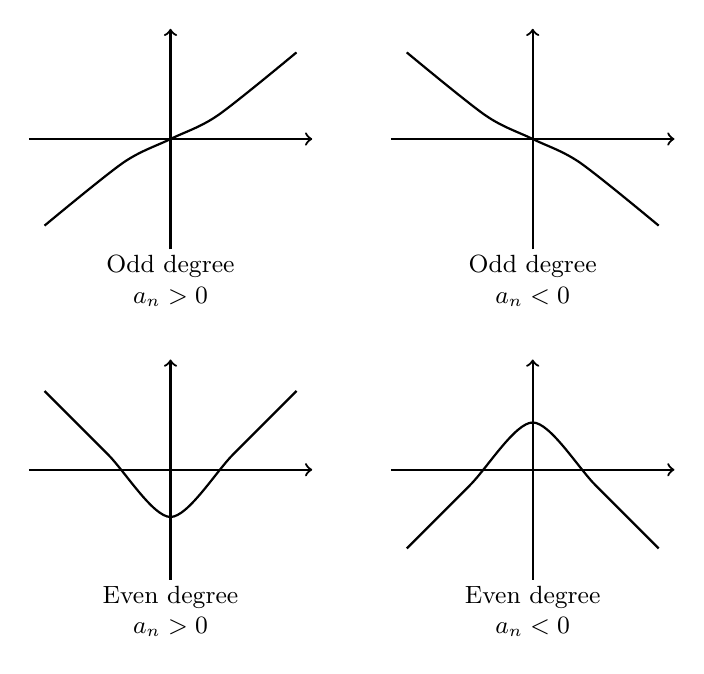
\begin{tikzpicture}[x=1cm,y=1cm]
    % A compact 2x2 summary of polynomial end behavior.
    % Each panel shows axes + a stylized curve (not a specific polynomial).

    \tikzset{
      axes/.style={->, thick},
      curve/.style={thick},
      label/.style={font=\small, align=center}
    }

    % --- Panel 1: odd degree, leading coefficient > 0 (down-left to up-right)
    \begin{scope}[shift={(0,0)}]
      \draw[axes] (-1.8,0) -- (1.8,0);
      \draw[axes] (0,-1.4) -- (0,1.4);
      \draw[curve] plot[smooth] coordinates {(-1.6,-1.1) (-0.6,-0.3) (0.0,0.0) (0.6,0.3) (1.6,1.1)};
      \node[label] at (0,-1.8) {Odd degree\\$a_n>0$};
    \end{scope}

    % --- Panel 2: odd degree, leading coefficient < 0 (up-left to down-right)
    \begin{scope}[shift={(4.6,0)}]
      \draw[axes] (-1.8,0) -- (1.8,0);
      \draw[axes] (0,-1.4) -- (0,1.4);
      \draw[curve] plot[smooth] coordinates {(-1.6,1.1) (-0.6,0.3) (0.0,0.0) (0.6,-0.3) (1.6,-1.1)};
      \node[label] at (0,-1.8) {Odd degree\\$a_n<0$};
    \end{scope}

    % --- Panel 3: even degree, leading coefficient > 0 (both ends up)
    \begin{scope}[shift={(0,-4.2)}]
      \draw[axes] (-1.8,0) -- (1.8,0);
      \draw[axes] (0,-1.4) -- (0,1.4);
      \draw[curve] plot[smooth] coordinates {(-1.6,1.0) (-0.8,0.2) (0.0,-0.6) (0.8,0.2) (1.6,1.0)};
      \node[label] at (0,-1.8) {Even degree\\$a_n>0$};
    \end{scope}

    % --- Panel 4: even degree, leading coefficient < 0 (both ends down)
    \begin{scope}[shift={(4.6,-4.2)}]
      \draw[axes] (-1.8,0) -- (1.8,0);
      \draw[axes] (0,-1.4) -- (0,1.4);
      \draw[curve] plot[smooth] coordinates {(-1.6,-1.0) (-0.8,-0.2) (0.0,0.6) (0.8,-0.2) (1.6,-1.0)};
      \node[label] at (0,-1.8) {Even degree\\$a_n<0$};
    \end{scope}
  \end{tikzpicture}
\end{center}

\vspace{1em}
\noindent\textbf{Examples: Determine the End Behavior}
\begin{enumerate}
    \item $f(x) = -3x^5 + 2x^2 - 7$
    \begin{itemize}
        \item \textbf{Leading Term:} $-3x^5$ (Degree = $5$ / Odd, $a_n = -3 < 0$)
        \item \textbf{End Behavior:} Opposite directions, Q2 $\to$ Q4.
        \item $\lim_{x \to -\infty} f(x) = \infty$, \quad $\lim_{x \to \infty} f(x) = -\infty$
    \end{itemize}
    
    \item $g(x) = 4x^4 - 5x^3 + x$
    \begin{itemize}
        \item \textbf{Leading Term:} $4x^4$ (Degree = $4$ / Even, $a_n = 4 > 0$)
        \item \textbf{End Behavior:} Same direction, both ends up (Q2 $\to$ Q1).
        \item $\lim_{x \to \pm\infty} g(x) = \infty$
    \end{itemize}

    \item $h(x) = -2x(x-3)^2(x+1)^3$ \quad \textit{(Watch out for factored form!)}
    \begin{itemize}
        \item \textbf{Leading Term:} Multiply highest powers of each factor: $-2x \cdot (x)^2 \cdot (x)^3 = -2x^6$
        \item \textbf{Analyze:} Degree = $6$ / Even, $a_n = -2 < 0$.
        \item \textbf{End Behavior:} Same direction, both ends down (Q3 $\to$ Q4).
        \item $\lim_{x \to \pm\infty} h(x) = -\infty$
    \end{itemize}
\end{enumerate}

\section{Domain, Range, and Symmetry}
\subsection{Domain}
All polynomials are defined for all real numbers: $D = \mathbb{R}$.

\subsection{Range}
\begin{itemize}
  \item Odd degree: $R = \mathbb{R}$
  \item Even degree: has a global max or min depending on leading coefficient
\end{itemize}

\subsection{Symmetry}
\begin{itemize}
  \item Even function: $f(-x) = f(x)$, symmetric about $y$-axis (contains only even powers)
  \item Odd function: $f(-x) = -f(x)$, symmetric about origin (contains only odd powers, no constant term)
\end{itemize}

\vspace{0.5em}
\noindent\textbf{Proof (Why Even Functions contain only even powers):} \\
Let $f(x) = ax^3 + bx^2 + cx + d$. If $f(x)$ is an even function, it must satisfy $f(-x) = f(x)$ for all $x$.
\begin{align*}
  f(-x) &= a(-x)^3 + b(-x)^2 + c(-x) + d \\
        &= -ax^3 + bx^2 - cx + d
\end{align*}
Equating $f(-x)$ and $f(x)$:
\[ -ax^3 + bx^2 - cx + d = ax^3 + bx^2 + cx + d \]
For this equation to hold true for \textit{all} $x$, the coefficients of corresponding powers must be equal:
\begin{itemize}
  \item For $x^3$: $-a = a \implies 2a = 0 \implies a = 0$
  \item For $x^1$: $-c = c \implies 2c = 0 \implies c = 0$ 
\end{itemize}
Thus, all odd power coefficients must be zero, leaving only even powers: $f(x) = bx^2 + d$. \\
\textit{(The same logic applies to Odd Functions, forcing even power coefficients and constant terms to zero).}

\vspace{0.5em}
\noindent\textbf{Important Note (Beyond Polynomials):} \\
The ``looking at powers'' shortcut works \textbf{only for polynomials}. The core definitions $f(-x) = f(x)$ and $f(-x) = -f(x)$ are universal and apply to \textbf{all functions} in mathematics!
\begin{itemize}
  \item \textbf{Even Functions}: $f(x) = \cos(x)$ or $f(x) = |x|$. They are perfectly symmetric about the $y$-axis, even though they aren't polynomials.
  \item \textbf{Odd Functions}: $f(x) = \sin(x)$ or $f(x) = \frac{1}{x}$. They are perfectly symmetric about the origin.
\end{itemize}
When encountering non-polynomials later in Calculus, you \textbf{must} return to the $f(-x)$ algebraic substitution method to test for symmetry!

\vspace{1em}
\noindent\textbf{Examples: Determine Domain, Range, and Symmetry}
\begin{enumerate}
    \item $f(x) = 2x^4 - 8x^2 + 3$
    \begin{itemize}
        \item \textbf{Domain:} $D = \mathbb{R}$ (True for all polynomials)
        \item \textbf{Range:} Even degree ($a_n > 0$) $\implies$ both ends up. It has a global minimum. By treating it as a quadratic in $x^2$, the minimum value is $-5$. Thus, Range = $[-5, \infty)$.
        \item \textbf{Symmetry:} Contains \textit{only} even powers ($x^4$, $x^2$, constant). It is an \textbf{Even Function} (Symmetric about the $y$-axis).
    \end{itemize}
    
    \item $g(x) = -x^5 + 4x^3$
    \begin{itemize}
        \item \textbf{Domain:} $D = \mathbb{R}$
        \item \textbf{Range:} Odd degree $\implies$ $R = \mathbb{R}$
        \item \textbf{Symmetry:} Contains \textit{only} odd powers ($x^5$, $x^3$) and no constant term. It is an \textbf{Odd Function} (Symmetric about the origin).
    \end{itemize}

    \item $h(x) = x^3 - 2x^2 + x$
    \begin{itemize}
        \item \textbf{Domain:} $D = \mathbb{R}$
        \item \textbf{Range:} Odd degree $\implies$ $R = \mathbb{R}$
        \item \textbf{Symmetry:} Contains a \textit{mix} of odd (3, 1) and even (2) powers. It is \textbf{Neither} even nor odd.
    \end{itemize}
\end{enumerate}

\newpage
\section{Zeros and Sign Intervals}
\begin{itemize}
  \item Zeros: solve $f(x) = 0$, points where graph intersects x-axis, at most $n$ real zeros.
  \item Positive intervals: $f(x) > 0$, graph above x-axis.
  \item Negative intervals: $f(x) < 0$, graph below x-axis.
\end{itemize}

\textbf{Procedure to find sign intervals}:
\begin{enumerate}
  \item Solve $f(x) = 0$ and mark zeros on number line.
  \item Divide the number line into intervals by zeros.
  \item Choose a test point in each interval, evaluate $f(x)$.
  \item If $f(x) > 0$, interval is positive; if $f(x) < 0$, interval is negative.
\end{enumerate}

\section{Examples: Sign Intervals}

\textbf{Example 1: A Standard Cubic (Factored Form)}
\[
  f(x) = (x+2)(x-1)(x-3)
\]

\textbf{Step 1: Find the Zeros}
\[
  f(x) = 0 \implies x = -2, 1, 3
\]

\textbf{Step 2: Number Line \& Test Points (Sign-Only Method)}
\begin{itemize}
  \item \textbf{Interval $(-\infty, -2)$}: Test $x = -3$. \\
  Signs: $(-)(-) (-) \implies \textbf{Negative}$
  
  \item \textbf{Interval $(-2, 1)$}: Test $x = 0$. \\
  Signs: $(+)(-) (-) \implies \textbf{Positive}$
  
  \item \textbf{Interval $(1, 3)$}: Test $x = 2$. \\
  Signs: $(+)(+) (-) \implies \textbf{Negative}$
  
  \item \textbf{Interval $(3, \infty)$}: Test $x = 4$. \\
  Signs: $(+)(+) (+) \implies \textbf{Positive}$
\end{itemize}
\textit{Conclusion:} Positive intervals: $(-2, 1) \cup (3, \infty)$. Negative intervals: $(-\infty, -2) \cup (1, 3)$.

\vspace{1em}
\textbf{Example 2: Negative Coefficient \& Standalone $x$}
\[
  g(x) = -2x(x+4)(x-2)
\]

\textbf{Step 1: Find the Zeros}
\[
  g(x) = 0 \implies x = 0, -4, 2
\]
\textit{(Graphing Tip: Always place them in numerical order: $-4, 0, 2$)}

\textbf{Step 2: Number Line \& Test Points}
\begin{itemize}
  \item \textbf{Interval $(-\infty, -4)$}: Test $x = -5$. \\
  Signs: $(-2)(-)(-) (-) \implies \textbf{Positive}$ \quad \textit{(4 minus signs $\implies$ +)}
  
  \item \textbf{Interval $(-4, 0)$}: Test $x = -1$. \\
  Signs: $(-2)(-)(+) (-) \implies \textbf{Negative}$ \quad \textit{(3 minus signs $\implies$ -)}
  
  \item \textbf{Interval $(0, 2)$}: Test $x = 1$. \\
  Signs: $(-2)(+)(+) (-) \implies \textbf{Positive}$ \quad \textit{(2 minus signs $\implies$ +)}
  
  \item \textbf{Interval $(2, \infty)$}: Test $x = 3$. \\
  Signs: $(-2)(+)(+) (+) \implies \textbf{Negative}$ \quad \textit{(1 minus sign $\implies$ -)}
\end{itemize}

\end{document}
